\documentclass[journel,12pt,twocoloums]{IEEEtran}

\title{Assignment 13-Probability and Random Variable}
\author{Annu-EE21RESCH01010}

\date{13 January 2020}

\usepackage{amsthm}
\usepackage{graphicx}
\usepackage{mathrsfs}
\usepackage{txfonts}
\usepackage{stfloats}
\usepackage{pgfplots}
\usepackage{cite}
\usepackage{cases}
\usepackage{mathtools}
\usepackage{caption}
\usepackage{enumerate}	
\usepackage{enumitem}
\usepackage{amsmath}
\usepackage[utf8]{inputenc}
\usepackage[english]{babel}
\usepackage{multicol}
%\usepackage{xtab}
\usepackage{longtable}
\usepackage{multirow}
%\usepackage{algorithm}
%\usepackage{algpseudocode}
\usepackage{array,multirow}
\usepackage{enumitem}
\usepackage{mathtools}
\usepackage{gensymb}
\usepackage{hyperref}
%\usepackage[framemethod=tikz]{mdframed}
\usepackage{listings}
    %\usepackage[latin1]{inputenc}                                %%
    \usepackage{color}                                            %%
    \usepackage{array}                                            %%
    \usepackage{longtable}                                        %%
    \usepackage{calc}                                             %%
    \usepackage{multirow}                                         %%
    \usepackage{hhline}                                           %%
    \usepackage{ifthen}                                           %%
  \providecommand{\nCr}[2]{\,^{#1}C_{#2}}
  \providecommand{\nPr}[2]{\,^{#1}P_{#2}}
  \lstset{
%language=C,
frame=single, 
breaklines=true,
columns=fullflexible
}
\usepackage{tikz}
\usetikzlibrary{shapes,arrows,positioning}
 \begin{document}
 \maketitle
\textbf{Download latex code from here-}\\
\begin{lstlisting}
 https://github.com/annu100/AI5002-Probability-and-Random-variables/tree/main.tex/ASSIGNMENT_13
 \end{lstlisting}

 \section{Gate-24 Solution}

A binary symmetric channel (BSC) has a transition
probability of $\frac{1}{8}$. If the binary transmit
symbol X is such that $Pr(X=0)=\frac{9}{10}$,then
the probability of error for an optimum receiver
will be-

\section{SOLUTIONS}
let crossover probability=$p$\\
\begin{figure}[h!]
    \centering
    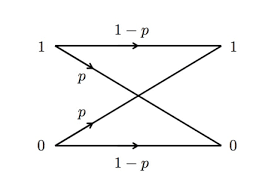
\includegraphics{channel_diag.png}
    \caption{Channel transition diagram}
    \label{fig:Channel transition diagram}
\end{figure}q
\begin{flushleft}
$x_0$=0,$x_1$=1,$y_0$=0,$y_1$=1 for binary channel\\
Let $x_0$ and $x_1$ are two binary transmitted symbols.\\
$y_0$ and $y_1$ are recieved symbols.\\
transition probability=$Pr(y_1|x_0)$=$Pr(y_0|x_1)$
Given data-\\
$Pr(x_0)=\frac{9}{10}$\\
$Pr(x_1)=1-\frac{9}{10}=\frac{1}{10}$\\
$Pr(y_1|x_0)=p=\frac{1}{8}$\\
$Pr(y_0|x_1)=p=\frac{1}{8}$\\
$Pr(y_0|x_0)=1-p=1-\frac{1}{8}=\frac{9}{10}$\\
$Pr(y_1|x_1)=1-p=1-\frac{1}{8}=\frac{9}{10}$\\
Calculating probability values for MAP critera -
\end{flushleft}

\begin{align}
 Pr(y_0|x_0) \times Pr(x_0) &= \frac{7}{8} \times \frac{9}{10} \\
                     &= \frac{63}{80}
\end{align}
\begin{align}
 Pr(y_0|x_1) \times Pr(x_1) &= \frac{1}{8} \times \frac{1}{10} \\
                     &= \frac{1}{80}
\end{align}
\begin{align}
 Pr(y_1|x_0) \times Pr(x_0) &= \frac{1}{8} \times \frac{9}{10} \\
                     &= \frac{9}{80}
\end{align}
\begin{align}
 Pr(y_1|x_1) \times Pr(x_1) &= \frac{7}{8} \times \frac{1}{10}\\
                     &= \frac{7}{80}
\end{align}
Now according to M.A.P criteria at reciever -\\
\begin{align}
Pr(y_0|x_0) \times Pr(x_0)>Pr(y_0|x_1) \times Pr(x_1)
\end{align}
So,when a symbol is recieved is recieved as $y_0$ ,the decision can be made in favour of $x_0$ in an optimum way.\\
\begin{align}
Pr(y_0|x_0) \times Pr(x_0)>Pr(y_0|x_1) \times Pr(x_1)
\end{align}
So,when a symbol is recieved is recieved as $y_0$ ,the decision can be made in favour of $x_0$ in an optimum way.\\
As\\
\begin{align}
Pr(y_0|x_0) \times Pr(x_0)>Pr(y_0|x_1) \times Pr(x_1)\\
=(1-p) \times \frac{9}{10}> p \times \frac{1}{10}
\end{align}
So,when a symbol is recieved is recieved as $y_0$ ,the decision can be made in favour of $x_0$ in an optimum way.\\
\begin{align}
Pr(y_1|x_0) \times Pr(x_0)>Pr(y_1|x_1) \times Pr(x_1)\\
=p \times \frac{9}{10}>(1-p) \times \frac{1}{10}
\end{align}
So,when a symbol is recieved is recieved as $y_1$ ,the decision can be made in favour of $x_0$ in an optimum way.\\
So,for the given BSC channel ,with optimum reciver ,both the recieved symbols will be decoded as $x_0$.\\
Hence,the probability of error is equal to probability of transmitting $x_1$.\\
so,$Pr(error)=Pr(x_1)=\frac{1}{10}$
\end{document}

        
